%!TEX root = ../../../thesis.tex
\chapter{Slime Mold Graph Repository}\label{chap:smgr}

	In this chapter we introduce the Slime Mold Graph Repository (\SMGR), a novel data collection promoting the visibility, accessibility and reuse of experimental data revolving around network-forming slime molds. By making data readily available to researchers across multiple disciplines, the \SMGR promotes novel research as well as the reproduction of original results. While \SMGR data may take various forms, we stress the importance of graph representations of slime mold networks due to their ease of handling and their large potential for reuse. Data added to the \SMGR stands to gain impact beyond initial publications or even beyond its domain of origin. 

	We initiate the \SMGR with the comprehensive \data focusing on the slime mold \Pp, which we obtained in the course of our original research. It contains sequences of images documenting growth and network formation of the organism under constant conditions. Suitable image sequences depicting the typical \P network structures are used to compute sequences of graphs faithfully capturing them. Given such sequences, node identities are computed, tracking the development of nodes over time. Based on this information we demonstrate two out of many possible ways to begin exploring the data. The entire data set is well-documented, self-contained and ready for inspection via the \SMGR at \href{http://smgr.mpi-inf.mpg.de}{http://smgr.mpi-inf.mpg.de}.

	The present chapter reports on joined work with Mag.~T.~Mehlhorn as well as Prof.~Dr.~K.~Mehlhorn. The former was responsible for the realization of all described wet-lab experiments in the laboratories of the Korea Institute of Science and Technology Europe (\href{www.kist-europe.de}{\textsc{Kist} Europe}).

\section{Introduction}

	Slime molds are interesting and complex organisms providing a rich substrate for interdisciplinary research. One member of the family, \Pp, has received increasing interest as of late resulting in intensive research efforts that continue to shed light on many aspects of this organism. Of particular interest is its ability to form and maintain complex networks. Efforts to improve our understanding of formation, structure and function of these networks are manifold~\cite{Marwan419,tero2010rules,alim2013random,baumgarten2010plasmodial,baumgarten2013functional} and ongoing.

 	A popular two-step approach, not restricted to slime molds, consists of taking images of the networks formed by the organism and converting them to graphs\footnote{In this context graphs denote abstract mathematical objects, subject of Graph Theory, consisting of vertices and edges. Throughout this thesis we will use both terms interchangeably}. First, images are obtained by cultivating \Pp in the wet-lab whilst documenting the development of the organism and its networks. This is a time consuming process which needs to be repeated sufficiently often under constant conditions to acquire a reliable body of observations. 

 	The second part requires methods capable of analyzing an image and deriving a faithful graph representation of the network depicted therein. Such methods have become available recently as convenient software packages~\cite{dirnberger2015nefi}. Once graphs are available, concepts and methods from Network Science and Graph Theory directly apply, enabling efficient and detailed investigations of graph properties~\cite{baumgarten2012computational,heaton2012analysis}.

 	We stress that both steps are challenging as they require time, special laboratory resources and expert knowledge. Data acquisition and graph extraction in particular, may quickly become serious obstacles deterring interested researchers from starting to work with networks formed by \P. 

 	Despite such difficulties, ``graph-based'' approaches have been quite successful and various interesting results are available today~\cite{baumgarten2010plasmodial,baumgarten2013functional,fessel2014analytical,fessel2012Physarum,ito2011characterization}. However, data used to establish these results, \ie the graphs and their underlying images themselves, are not nearly as available in many cases. This is unfortunate because due to their ease of handling and their abstraction power, graphs naturally lend themselves to reuse, potentially gaining impact beyond their initial publications or even beyond their domain of origin.

 	Our own experience shows, that most researchers are, at least in principle, willing to share their valuable data. However, data sharing can be cumbersome and constitutes an extra hurdle discouraging data reuse. To combat this, data needs to be collected and made available in an organized fashion. Similar efforts have become best practice for diverse types of data originating in various fields of science. Examples are numerous including collections of images of cells~\cite{cell}, large graphs~\cite{snap} or experimental data in high energy physics~\cite{hepdata}, to name but a few.

	To the best of our knowledge no such repository exists for data concerned with networks of slime molds. For this reason we decided to set up the \emph{Slime Mold Graph Repository} with the goal of providing an available collection of networks focused on slime molds. Although this is clearly a niche topic, we believe that due to the many open question revolving around the structure and function of such networks and their large interdisciplinary appeal, setting up a small but dedicated repository is of pronounced value.

	In the following we discuss the concept and benefits of the \SMGR followed by detailed account of its initial contents, the \data. We start by discussing how the data was obtained experimentally and move on to present our tracking algorithm, a novel method designed to resolve how networks formed by \P change in time. To illustrate the usefulness of both data and method, we show proof-of-principle applications which suggest avenues for further research. Our exposition aims to promote the \SMGR across disciplines and is sufficiently detailed for non-experts to access.
	
\section{Repository Concept and Benefits}
	
	Today the impact of data sharing as a scientific practice is ever increasing. Currently, two major forms of data collections are commonly encountered.

	First, data is collected in large, well-organized repositories holding enormous amounts of information. Such major repositories easily contain thousands of datasets, covering numerous topics across its domain of relevance. Due to their size and complexity, curating and maintaining such repositories requires major resources typically provided by larger research institutions or non-profit organizations. 

	Most major data collections, however, have started as small and specialized repositories at some point. Such repositories constitute the second approach to data sharing common today. These are typically much simpler in structure and contain a smaller number of datasets. Small repositories tend to be more specialized and have very close ties to their relevant research communities since the operators of the repository are often researchers themselves. Their small size allows them to operate with minimal infrastructure requirements since changes to the repository are less frequent and data sets are limited in number and space requirements. Due to their minimal implementation they do not offer most of the services frequently provided by larger repositories and focus on but the most essential features.

	With the \SMGR we seek to establish a collection of research-grade data revolving around network-forming slime molds. Given the highly specialized nature of the topic, we believe that setting up a small stand-alone repository realized as a minimal implementation is advantageous and the correct point to start from. Note that we do not present novel software but rather combine available open source software components to supply a minimal repository service. Keeping the repository simple allows for easier maintenance and more flexibility. As a result it is easier to adapt and evolve based on community feedback. This is why at present only the most basic features necessary for repository operation are offered by the \SMGR. However, if sufficient and continued interest is observed, the implementation of additional features may be warranted. For further reasons why we launch the \SMGR as a minimal repository, please consult the FAQ on the \href{http://smgr.mpi-inf.mpg.de}{\SMGR project page}. 

	In its present form, the idea of the \SMGR was first introduced at \emph{PhysNet 2015} in New York and was well received with individuals signaling their willingness to contribute data~\cite{physnet2015}. We strongly believe that a tight integration with the research community, is key to the future success of the \SMGR. 

	The benefits of the \SMGR are manifold. Making data available for everyone increases visibility of contributors, allows original results to be reproduced and puts data in a prime position to become a catalyst for novel research. Given the significant costs, \ie time and resources, which are typically associated with obtaining high quality data, promoting increased reuse of data is an economical choice. Researchers and other professionals that do not have the required resources/connections to produce/obtain their own data sets benefit in particular from repositories like the \SMGR, since it provides immediate and convenient access to experimental material that would be hard to acquire by other means. 

	We envision the \SMGR to become a mediator between theory and experiment. Theoretical work in biology and biophysics concerned with modeling various aspects of \P networks, may utilize experimental data as a testbed for model predictions. This approach has been put into practice previously~\cite{baumgarten2015network}, but was exclusive to researchers in possession of relevant data. With the introduction of the \SMGR such limitations are removed. Similar statements can be made for other fields, \eg Computer Science, which is actively studying \P in the context of Natural Computing. Access to experimental data via the \SMGR allows to compare theory and experiment and to build the intuition crucial to theoretical investigations and modeling efforts. 

 	In order for the \SMGR to be useful from day one, we initiate the repository by sharing the extensive data that is driving our own slime mold research which was obtained at the \emph{Korea Institute of Science and Technology Europe} in Saarbr\"ucken. It is important to us, that anyone can go the \SMGR project page, download our data and immediately start working with it in whichever way he or she chooses. The data set we provide also serves as a possible example for the type of data the \SMGR intends to collect and what level of documentation is appreciated. 

 	We stress at this point that the \SMGR is not intended to simply function as long-time data storage. First and foremost, we seek to collect data that has not yet been fully explored or has a strong potential to be of use to others. The \data fulfills both criteria.

	Finally, any repository needs a set of instructions, policies and requirements applying to data submission, data usage and various other general aspects of repository operation. For these the \SMGR relies on established best practices of data sharing whilst striving to keep things as straight-forward as possible~\cite{white2013nine}. A detailed account can be found on the \href{http://smgr.mpi-inf.mpg.de}{\SMGR project page}, which we consider an integral part of this contribution. We opt to treat policies, user instructions and other important questions in a comprehensive FAQ on the \href{http://smgr.mpi-inf.mpg.de}{\SMGR project page} rather than in this thesis, simply because they are subject to future change.

	The \SMGR and all available data can be found here: \href{http://smgr.mpi-inf.mpg.de}{http://smgr.mpi-inf.mpg.de}. 

\section{The KIST Europe Data Set}	

	In the following we present an overview of the \data designed to give the interested reader a high-level understanding of its nature and content. At the same time, we recommend to inspect the data directly using the browsing and download functions provided on the \href{http://smgr.mpi-inf.mpg.de}{\SMGR project page}. We refer the expert reader, interested in reproducing all the steps involved in the creation of the data set, to an in-depth exposition given in \Fref{app:smgr}.

	The \data contains raw and processed data obtained and derived from $81$ identical wet-lab experiments, carefully executed under constant conditions. \Fref{fig:setup} illustrates the experimental setup used. The data was produced using the following procedure:

	\begin{enumerate}
		\item A rectangular plastic dish is prepared with a thin sheet of \SI{1.25}{\percent} agar.
		\item \SI{1.5}{\gram} of dried \P (HU195xHU200) sclerotia crumbs are lined up along the short edge of the dish, see \Fref{fig:sequence_1}. The dish is put into a large light-proof box.
		\item After approximately \SI{14}{\hour} the plasmodium resuscitates and starts exploring the available space towards the far side of the dish. Typically, the apical zone needs to cover a distance of several centimeters before network formation can be observed properly, see \Fref{fig:sequence_2}.
		\item For the next \SI{30}{\hour} we take a top-view image of the growing plasmodium and the changing network every \SI{120}{\second} from a fixed position. A typical obtained image is seen in \Fref{fig:sequence_3}. We stop capturing when the apical zone is about to reach the far side of the dish, which is well outside of the observed area. 
		\item After obtaining sequences of images showing the characteristic networks of \P, we use \NEFI to compute corresponding sequences of graph representations of the depicted structures within a predefined region of interest~\cite{dirnberger2015nefi}, see \Fref{fig:sequence_4}. The graphs store precise information of the length and width of the edges as well as the coordinates of the nodes in the plane. A typical resulting unfiltered graph is seen in \Fref{fig:sequence_5}.
		\item Given the resulting sequence of graphs we apply filters removing artifacts and other unwanted features of the graphs. Then we proceed to compute a novel node tracking which encodes the time development of every node taking into account the changing topology of the evolving graphs.
	\end{enumerate}

	\begin{figure}
		\centering
		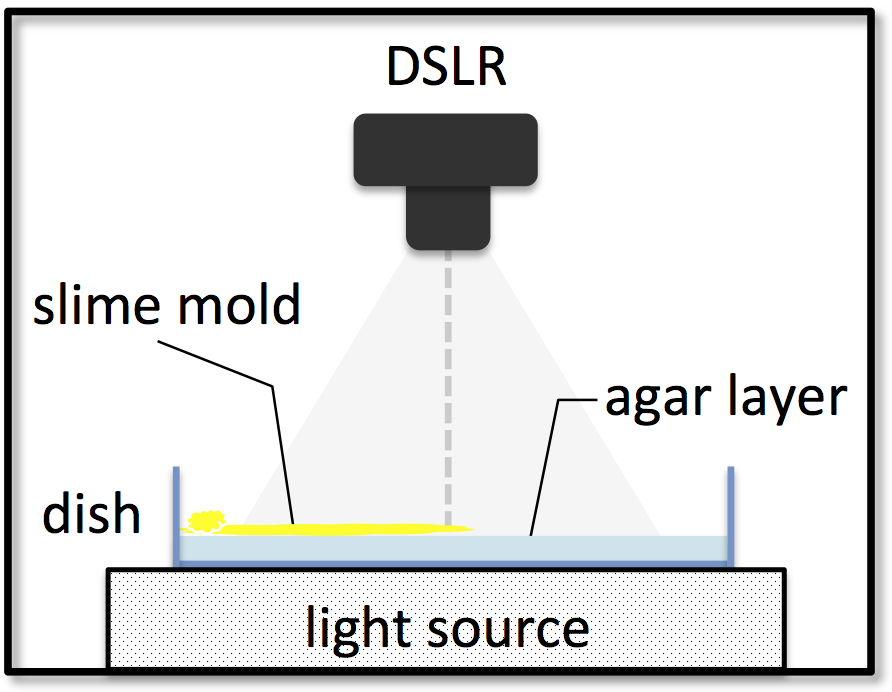
\includegraphics[width=0.5\linewidth,keepaspectratio]{setup.png}
		\caption[Setup for wetlab experiments.]{Schematic description of the experimental setup.}
		\label{fig:setup}
	\end{figure}

	\begin{figure}
		\centering
		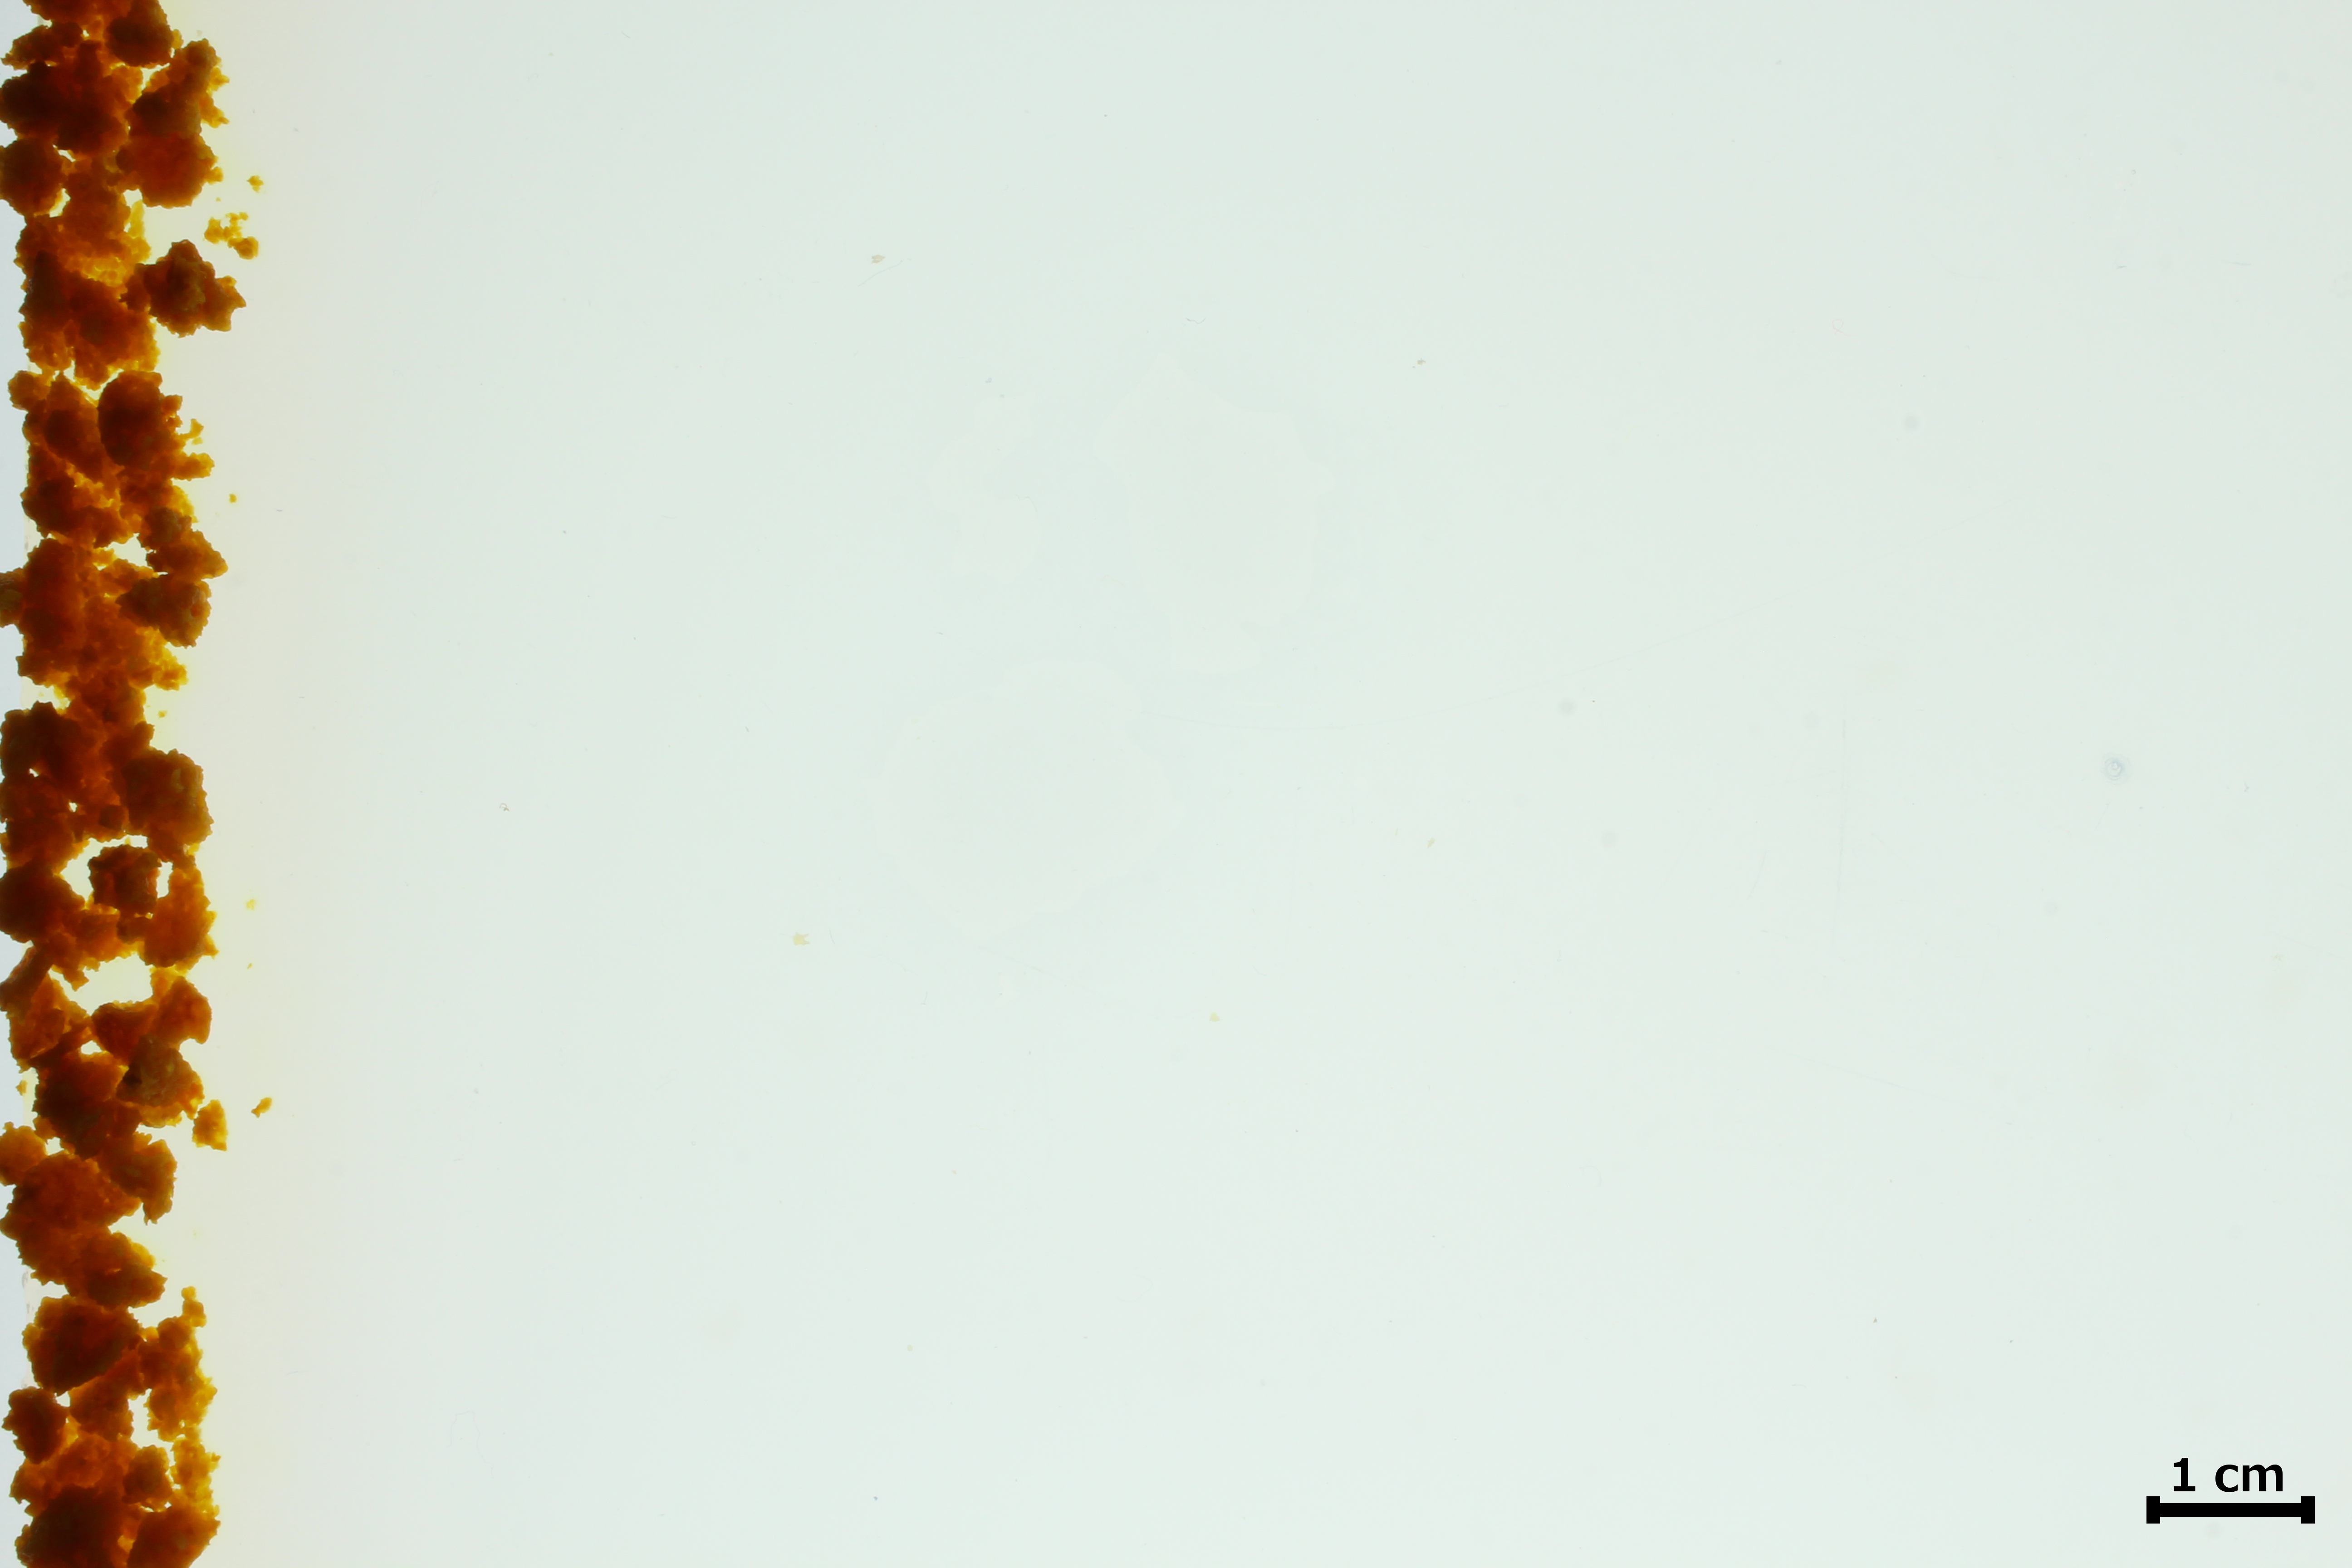
\includegraphics[width=0.5\linewidth,keepaspectratio]{physarum_sequence_1.JPG}
		\caption[Crumbs of \P sclerotia forming an inoculation line.]{Crumbs of \P sclerotia forming the inoculation line.}
		\label{fig:sequence_1}
	\end{figure}

	\begin{figure}
		\centering
		\includegraphics[width=0.5\linewidth,keepaspectratio]{physarum_sequence_2.JPG}
		\caption[The apical zone advances.]{The plasmodium explores the dish. The apical zone advances towards the right side of the dish supported by a complex network that is continuously forming.}
		\label{fig:sequence_2}
	\end{figure}

	\begin{figure}
		\centering
		\includegraphics[width=0.5\linewidth,keepaspectratio]{physarum_sequence_3.JPG}
		\caption[The onset of network coarsening.]{As the apical zone is about to escape the observation region, the coarsening of the network becomes more pronounced.}
		\label{fig:sequence_3}
	\end{figure}

	\begin{figure}
		\centering
		\includegraphics[width=0.5\linewidth,keepaspectratio]{physarum_sequence_4.JPG}
		\caption[A complex network of veins within a region of interest.]{The apical zone has moved on, leaving behind a complex network of veins. The dashed rectangle depicts a typical region of interest relevant for subsequent image analysis and graph detection.}
		\label{fig:sequence_4}
	\end{figure}

	\begin{figure}
		\centering
		\includegraphics[width=0.5\linewidth,keepaspectratio]{physarum_sequence_5.JPG}
		\caption[Graph extracted from the sample region of interest.]{The network within the region of interest has been extracted by \NEFI. Note that no filters have been applied. Dead ends and nodes of degree 2 are visible still, leading to small patches of nodes appearing to clump up. Such artifacts can be removed in suitable post-processing steps.}
		\label{fig:sequence_5}
	\end{figure}

	Repeating this experiment we obtain $81$ similar sequence of images, which we consider our raw data. We stress at this point that given the inherently uncontrollable growth process of \P, the obtained sequences differ in length and nature. In some experiments the organism behaved unfavorably, simply stopping its growth, changing direction or even escaping the container. While such sequences are part of the raw dataset, we excluded them partially or completely from the subsequent graph extraction efforts. The removal of such data reduces the number of series depicting optimal network formation to $54$.

	After obtaining the raw data, we transform the images into equivalent mathematical graphs, thus opening up a wealth of possibilities for data analysis. To this end we deploy \NEFI~\cite{dirnberger2015nefi}, which analyzes a digital image, separates the depicted slime mold network from the background and returns its graph representation. Using this tool effectively requires moderate amounts of image preprocessing. In particular, for each sequence of images it is necessary to decide on a suitable subsequence to be processed. Here we typically exclude parts of the sequence where the apical zone is still visible. For each such subsequence a suitable region of interest is defined manually. \Fref{fig:sequence_4} depicts a typical choice for the region of interest to be processed by \NEFI. The established unfiltered graph can be seen in \Fref{fig:sequence_5}. The graph stores the position of the nodes in the plane as well as edge attributes such as edge length and widths for each edge. In addition to the output of \NEFI including the unfiltered graphs, the dataset contains \NEFIs input, \ie the selected subsequences of images cropped according to their defined regions of interest.

	Note that some parts of the image series showing proper network formation did not yield optimal representations of the depicted networks. This is a result of images exhibiting strong color gradients or other effects rendering them too challenging for automatic network extraction. While such cases may still be handled by tuning the parameters of image processing manually on an image per image basis, we decided to discard affected series from subsequent processing efforts. As a result the number of usable graph sequences of highest quality reduced to $36$. To this we apply a set of filters removing artifacts, isolated small components and dead-end paths. Thus we obtain a total of $3134$ distinct filtered graphs faithfully reflecting the topology and edge attributes that \P displayed during the wet-lab experiments. 

	At this point available graph analysis packages or custom written analysis code can be deployed to investigate the data in various ways, \eg~\cite{ICWSM09154,schult2008exploring}. The dataset includes the filtered graphs as well as all corresponding graph drawings. The latter enable a quick visual inspection of the graph extraction results.

	Given the obtained time-ordered sequences of graphs the development of the entire graph can be investigated. One may also study what happens to single nodes as \P evolves. Given a graph in a sequence of graphs, let us pick any node $u$. Can we determine a set of nodes from graphs in the sequence that are equivalent to $u$, \ie all nodes in the set are earlier or later versions of $u$ in time? We answer this question by computing a so-called \emph{node tracking} which establishes the time development of all nodes in the graph. Crucially, this tracking takes into account topological changes in the evolving graphs. The result of the tracking is available as node properties of the graphs. Naturally, the program computing the tracking is included in the dataset. To the best of our knowledge, this type of data is made available for the first time through the \data.

	Finally, in addition to the actual data, \ie images and graphs, the \data contains scripts and larger programs used to process and evaluate the data. Suitable configuration files specify the used regions of interest and the parameters used with \NEFI. Thus it is possible to repeat the entire data production process from the raw images to the obtained filtered graphs including the tracking of nodes. As part of the \SMGR, the \data is well-structured and self-contained. In particular, sufficient on-the-fly documentation is available when using the online browsing function of the \SMGR.

	\subsection{Node Tracking}

		In this section we explain how to compute a node tracking. Our approach is a variant of a tracking method introduced previously~\cite{woll2013novel,Karrenbauer2013}. Here we give a self-contained account of the tracking technique geared towards non-experts in optimization. For technical details, proofs and an experimental evaluation of the method we refer the interested reader to the original publications.

		For each of our experiments, let us denote the respective time ordered sequence of $k$ filtered graphs with $\mathcal{G} = {G_1, G_2, \dots, G_t, \dots, G_k}$ and the union of the respective node sets with $\bar{V} = \bigcup_{i=1}^{k} V_{k}$. Each node in $\bar{V}$ can be represented as a non-negative integer triple $(x,y,t)$. Here $x$ and $y$ denote a node's pixel coordinates relating to the input image used for graph extraction and $t$ denotes its position in the sequence, \ie in time.

		We seek to exploit this information to partition the set $\bar{V}$ into a collection of disjoint, time-ordered paths such that every $u \in \bar{V}$ is part of exactly one path. We call such a path a \emph{track} and assign an unique identifier to it, \eg a unique color, which is shared by all nodes in the track. Intuitively speaking, rather than thinking of a track as a collection of nodes, one can interpret it as one physical node observed at different points in time.

		Let us define the length of a track by the number of nodes it contains. We stress that in general a track need not have length $k$. Tracks may start at any $t=i$ such that $1 \le i \le k$ and end at any $t=j$ such that $i \le j \le k$. In particular tracks of length $1$ are possible. Crucially, any node in a track has at most one predecessor and at most one successor node.

		Let us refer to the edges within a track as \emph{tracking edges}. Tracking edges may connect nodes of temporal distance larger than one, \ie:

		\begin{equation*}
			e = (u,v) = ((x_u,y_u,t_u), (x_u,y_u,t_v)) \qquad \text{and} \qquad 1 \le t_u < t_v \le k.
		\end{equation*}

		Such tracks simply ``skip'' nodes between the start and the endpoint of the track and correspond to nodes that have not been observed by \NEFI for some amount of time. Given the continued changes in the network topology observed during the growth of \P such tracks are expected to appear frequently. 

		Let us elaborate on two effects that impact said topology. First, \P networks tend to coarsen as time goes by. Eventually, this process may cause the thickness of receding veins to slowly drop below the detection threshold of \NEFI. Hence, they disappear from the graphs leading to tracks of length much shorter than $k$. Second, periodic changes in the thickness of veins are observed. It may happen that the thickness of a subset of contracting veins may drop below the detection threshold of \NEFI. As a result, those veins disappear from the graph. However, as the contraction cycle of the vein proceeds its thickness may increase again, eventually exceeding the detection threshold and thereby returning to the graph. These periodic changes in the topology of the graphs naturally lead to tracks that skip a certain number of frames periodically. Both effects are present at the same time and can be observed in the graphs we have obtained.

		We stress at this point that given a time resolution of \SI{120}{\second}, one must not use the graphs contained in the \data to study the sinusoidal behavior of edge thickness due to peristaltic pumping. The period of pumping is known to be approximately \SI{100}{\second} and can thus not be properly resolved~\cite{stewart1959protoplasmic}. However, changes in topology are on a much slower time scale and are reliably reflected by the graphs.

		We proceed to explain how to compute a node tracking. Let us study the graph in \Fref{fig:tracking} to gain some insight into the problem. Consider \eg node $a_1$. We seek to find a unique track that contains this node, representing its development in time. A straight-forward suggestion would be a track $T_a = [a_1,a_2,a_3]$. However the track $T_a = [a_1,c_2,f_3]$ is just as valid, as is $T_a = [a_3]$ and so forth. The example illustrates that the number of possible tracks and therefore the number of disjoint partitions into tracks grows exponentially with the number of nodes involved. 


		\begin{figure}
		\includestandalone[width=.3\textwidth]{tracking/tracking_1}
		\includestandalone[width=.3\textwidth]{tracking/tracking_2}
		\includestandalone[width=.3\textwidth]{tracking/tracking_3}
		\caption[Schematic description of node tracking.]{Schematic of a graph and its changing topology with respect to time. At time $t=2$ the edge $(b,e)$ and its nodes disappear from the graph because the thickness of the corresponding vein in \P dropped below the detection threshold of \NEFI. The colors indicate tracks $T_b$ and $T_e$ for nodes $b$ and $e$ respectively.}
		\label{fig:tracking}
		\end{figure}

		Ultimately, we seek to find a partition, that faithfully captures the time development of the nodes in $\bar{V}$. To do so we rely on the observation that optimal tracks are likely to consist of nodes that are close in space as well as close in time. In the following we formalize this requirement and construct a linear program (LP) that selects an optimal partition amongst all possible partitions. Once an LP has been defined, solving it becomes a standard task of optimization and can be done efficiently using solvers like Gurobi~\cite{optimization2012gurobi} or Cplex~\cite{cplex2005high}.

		Let us define the optimization problem we want to solve. First, we construct all possible tracking edges using space partition techniques. Assigning a unique identifier to each edge we obtain the set $\bar{E}$. When the linear program considers edges to include in a possible tracking solution it refers to them using the ids in this set. We define the cost of selecting a particular tracking edge $e = (u,v) = ((x_u,y_u,t_u), (x_v,y_v,t_v))$ as

		\begin{equation}
		\Delta(e) = \epsilon ((x_u - x_v)^2 + (y_u - y_v)^2 ) + \tau (t_u - t_v)^2,
		\end{equation}
		where $\epsilon$ and $\tau$ are constants used to control the relative strength of the squared Euclidean distance in space and time respectively. Note that using this cost function in our example in \Fref{fig:tracking}, track $T_a = [a_1,a_2,a_3]$ is favored over $T_a = [a_1,c_2,f_3]$. Note also that tracks of length $1$ have cost $0$ since there are no tracking edges to pay for. As a result the minimum cost solution consists of singleton tracks and is not very useful. To circumvent this problem we assign dedicated costs to any node that starts or ends a track as

		\begin{equation}
		p(u) = C.
		\end{equation}

		Here it is important that $C$ is selected carefully. It must not be too small since this will force the formation of artificial singleton tracks while too large a value may erroneously suppress such tracks. Going back to \Fref{fig:tracking}, assuming $\epsilon = \tau = 1$, a choice of $ 1 < C < 2^2 = 4$ will lead to two singleton tracks for the node $b$, namely ${b_1}$ and ${b_3}$ because a tracking edge connecting $b_1$ and $b_3$ comes at an edge cost of $\Delta(e)=4$. Increasing the node cost such that $C>2^2 = 4$ changes the picture and results in the desired tracks $T_b = [b_1, b_3]$ and $T_e = [e_1, e_3]$. The example illustrates the importance of the constants involved in the cost functions.

		Note that, we are still facing an exponential number of tracks to consider. Luckily, we can reduce the size of the set $\bar{E}$, and thus the size of the LP, dramatically by combining the effect of the costs functions with additional assumptions that valid for tracking \P graphs. In particular, the cost functions imply that we favor non-singleton tracks with nodes that are close in time as well as space. As a result, we may discard all options that have a geographical distance larger than a certain $R$ and a temporal distance larger than a certain $T$. Intuitively, when trying to find all possible tracking edges for a node $u$, we likely need not consider nodes that are located on the other side of the graph or have an unrealistically large temporal separation. Instead we can restrict the search to tracking edges within a cylinder centered at $u$ with radius $R$ and a height of $T$. We can exclude all tracking edges outside such a search cylinder, because their resulting costs are such that the linear program will never select any of them. 

		The problem thus boils down to determining suitable values for $R$ and $T$. Since the nodes of \P are well-separated and do not move within a time period of \SI{120}{\second}, a small radius of $R = \SI{30}{\pixel}$ is justified. We choose $T = 10$ which amounts to a time period of \SI{1200}{\second} to look for tracking edges in temporal direction. To tie the cost of singleton tracks to the physical features of our experiment, we choose $ C = 2 R^2 + T^4$. Setting $\epsilon =1$ and $\tau = 10$ completes the set of constants involved in the tracking problem. With these choices we follow the approach in~\cite{Karrenbauer2013}.

		We convinced ourselves that these settings are suitable for dealing with \P graphs by computing node trackings on artificial test graphs which enable a comparison with known ground truths. To obtain one such series we take a real \P graph and randomly remove a certain fraction of nodes from it to obtain artificial graphs at later times. Furthermore we slightly perturb the coordinates of all the nodes of these graphs. As expected we find the error rate to strongly depend on the strength of the geographical perturbation of nodes. As long as the perturbation is smaller than the minimum distance between nodes, the computed tracking is identical to the ground truth. When nodes start moving more from frame to frame, there is a danger that they randomly move past each other. As a result they end up swapping their respective tracks introducing an error. When the perturbation is set such that a node can only move within a radius of $R = \SI{30}{\pixel}$, less than \SI{4}{\percent} of the nodes end up in wrong tracks given the settings illustrated above. However, we expect that this error is somewhat pessimistic because nodes in real \P do not move much compared to our artificial test graphs. Careful visual inspection of the obtained node trackings resulting from real \P data supports this conjecture.

		From the arguments in the previous section it also follows that filtering has a strong impact on the quality of the node tracking. If graphs are filtered such that nodes are well-separated, excellent results can be expected. Thus, we recommend to carefully apply filters if any research questions based on the node tracking are to be tackled. In particular, contracting nodes of degree 2 is strongly advised.

		Finally, by combining the considerations discussed above, we are in a position to define the actual linear program computing a node tracking:

		\begin{alignat*}{4}
		minimize & : & \ \ f = &\sum_{ e \in \bar{E} } \Delta(e) x_{e}  &+  \sum_{ i \in \bar{V}} p(i) y_{i} & +   \sum_{ \substack{j \in \bar{V}}} p(j) z_{j} &  
		\end{alignat*}

		\begin{alignat*}{3}
		  s.t.:
		        & \ \     & \forall \ e \in \bar{E} : \ x_{e} \ge 0  \quad \quad    & \forall \ i \in \bar{V} : \ y_{i} \ge 0                                          & \forall \ j \in \bar{V} : \ z_{j} \ge 0                                             \\
		        & \ \     & \forall \ i: \ y_{i} = 1 - \sum_{e = (n,i) \in \bar{E}} x_{e}                                          &                                                     & \forall \ j: \ z_{j} = 1 - \sum_{e = (j,n) \in \bar{E}} x_{e}                     
		        % & \ \     & \forall \ e \sum_{f} y_{ef} \leq 1                                          &                                                     & \forall \ f \sum_{e} y_{ef} \leq 1                \\
		        % & \ \     & \overline{x}_{i} =  1 - \sum_{j \in V_B} x_{ij}                                &                                                     & \overline{x}_{j} =  1 - \sum_{i \in V_A} x_{ij}      \\          
		        % & \ \     & \overline{y}_{e} =  1 - \sum_{f \in E_B} y_{ef}                                &                                                     & \overline{y}_{f} =  1 - \sum_{e \in E_A} y_{ef}               
		        % % & \ \     &  \forall e = (a,b), f = (a',b') & & & 2y_{ef} \leq x_{aa'} + x_{ab'} + x_{ba'} + x_{bb'}                                                                 
		\end{alignat*}

		Note the last two constraints including sums over tracking edges that leave respectively enter a node. They make sure that a given node represented by $y_i$ either has exactly one predecessor or pays the cost $p(i)$ for starting a new track. Likewise, a node represented by $z_j$ either has exactly one successor or pays the cost $p(j)$ for ending an existing track. Thus the LP either pays for selecting a tracking edge or the penalties associated with ending or starting tracks but never both. For a more technical exposition of this optimization problem we refer the reader to~\cite{Karrenbauer2013}.

		The optimal values of the LP variables $x_e$, $y_i$ and $z_j$ are then determined by solving the LP. All LP variables are integer values automatically where a selected tracking edge $e$ is encoded by $x_e=1$, a selected node $i$ is starting a track if $y_i=1$ and ending it if $z_i=1$. Naturally, if $y_i=z_i=1$ we have a singleton track consisting solely of node $i$.

		Partitioning the entire selection into disjoint tracks yields the desired node tracking. As a final step, we assign each track a unique color identifier and propagate this color to each node in the track, \ie across all graphs in a given series. The color information is part of the graphs of all our datasets and thus readily available for further processing. A program constructing and solving this LP using Cplex~\cite{cplex2005high} is provided as part of the data set.

\section{Sample Usage of the KIST Europe Data Set}

	Next we illustrate the principal usefulness of the data contained in the \data set by demonstrating how to compute two different observables. The python code used to obtain the presented plots is available as part of the data set. As sample data we choose a time series of \P graphs consisting of $60$ graphs. Since the time between two graphs is \SI{120}{\second}, the whole series documents the growth of the slime mold for two hours. \Fref{fig:graph} shows one of the graphs superimposed on the image from the laboratory it was extracted from. The intricate network formed by \P is clearly visible. In particular it can be seen that the edges of the graph are of varying thickness. This is to be expected and reflects the variations of thickness observed in the veins of the slime mold. 

	One may ask the question of how the thickness of veins is distributed in these graphs. Answering this question is very easy, since the graphs in the \data all come with edge weights readily available. \ie edge thickness or lengths are present for all edges in the graphs. As a result the edge width data can easily be accessed an represented as a histogram. \Fref{fig:histogram} shows a cumulative normalized histogram of the edge widths including the edges from all $60$ graphs in the series. Note that the width is measured in \si{\pixel}. Due to the resolution of the original images \SI{37.0625}{\pixel} correspond to \SI{1}{\milli\metre} in the Petri dish.

	\begin{figure}[!htp]
		\centering
        \subfloat[]{%
		\label{fig:graph}%
		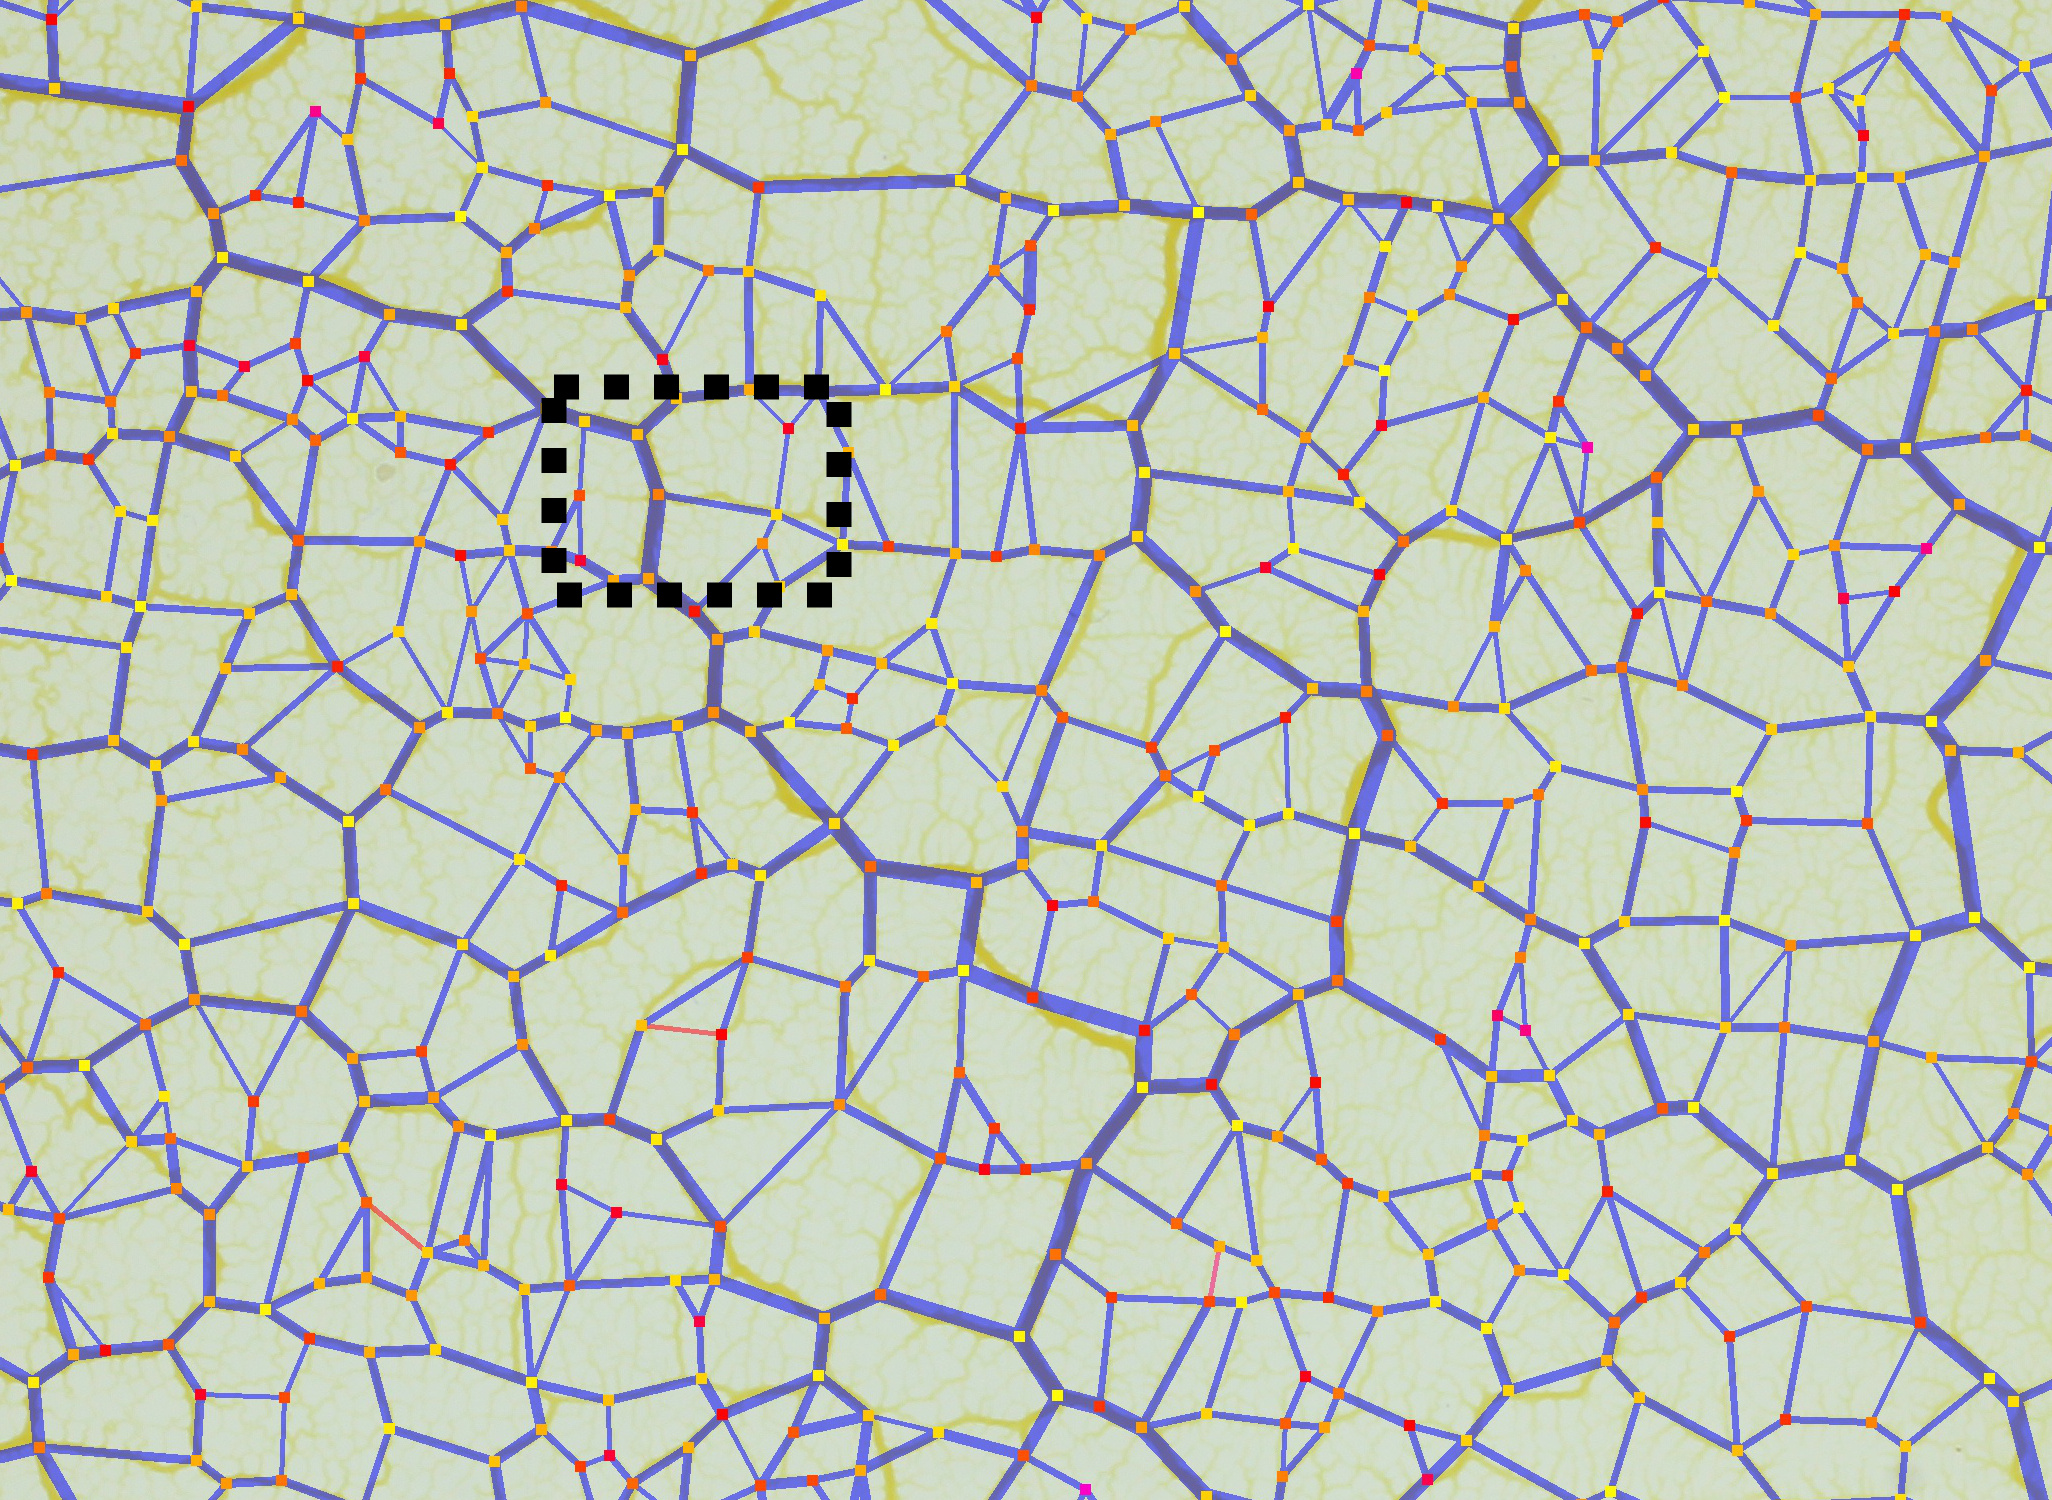
\includegraphics[width=0.45\textwidth]{demos/supergraph_10.jpg}}%
		\qquad
	    \subfloat[]{%
		\label{fig:histogram}%
		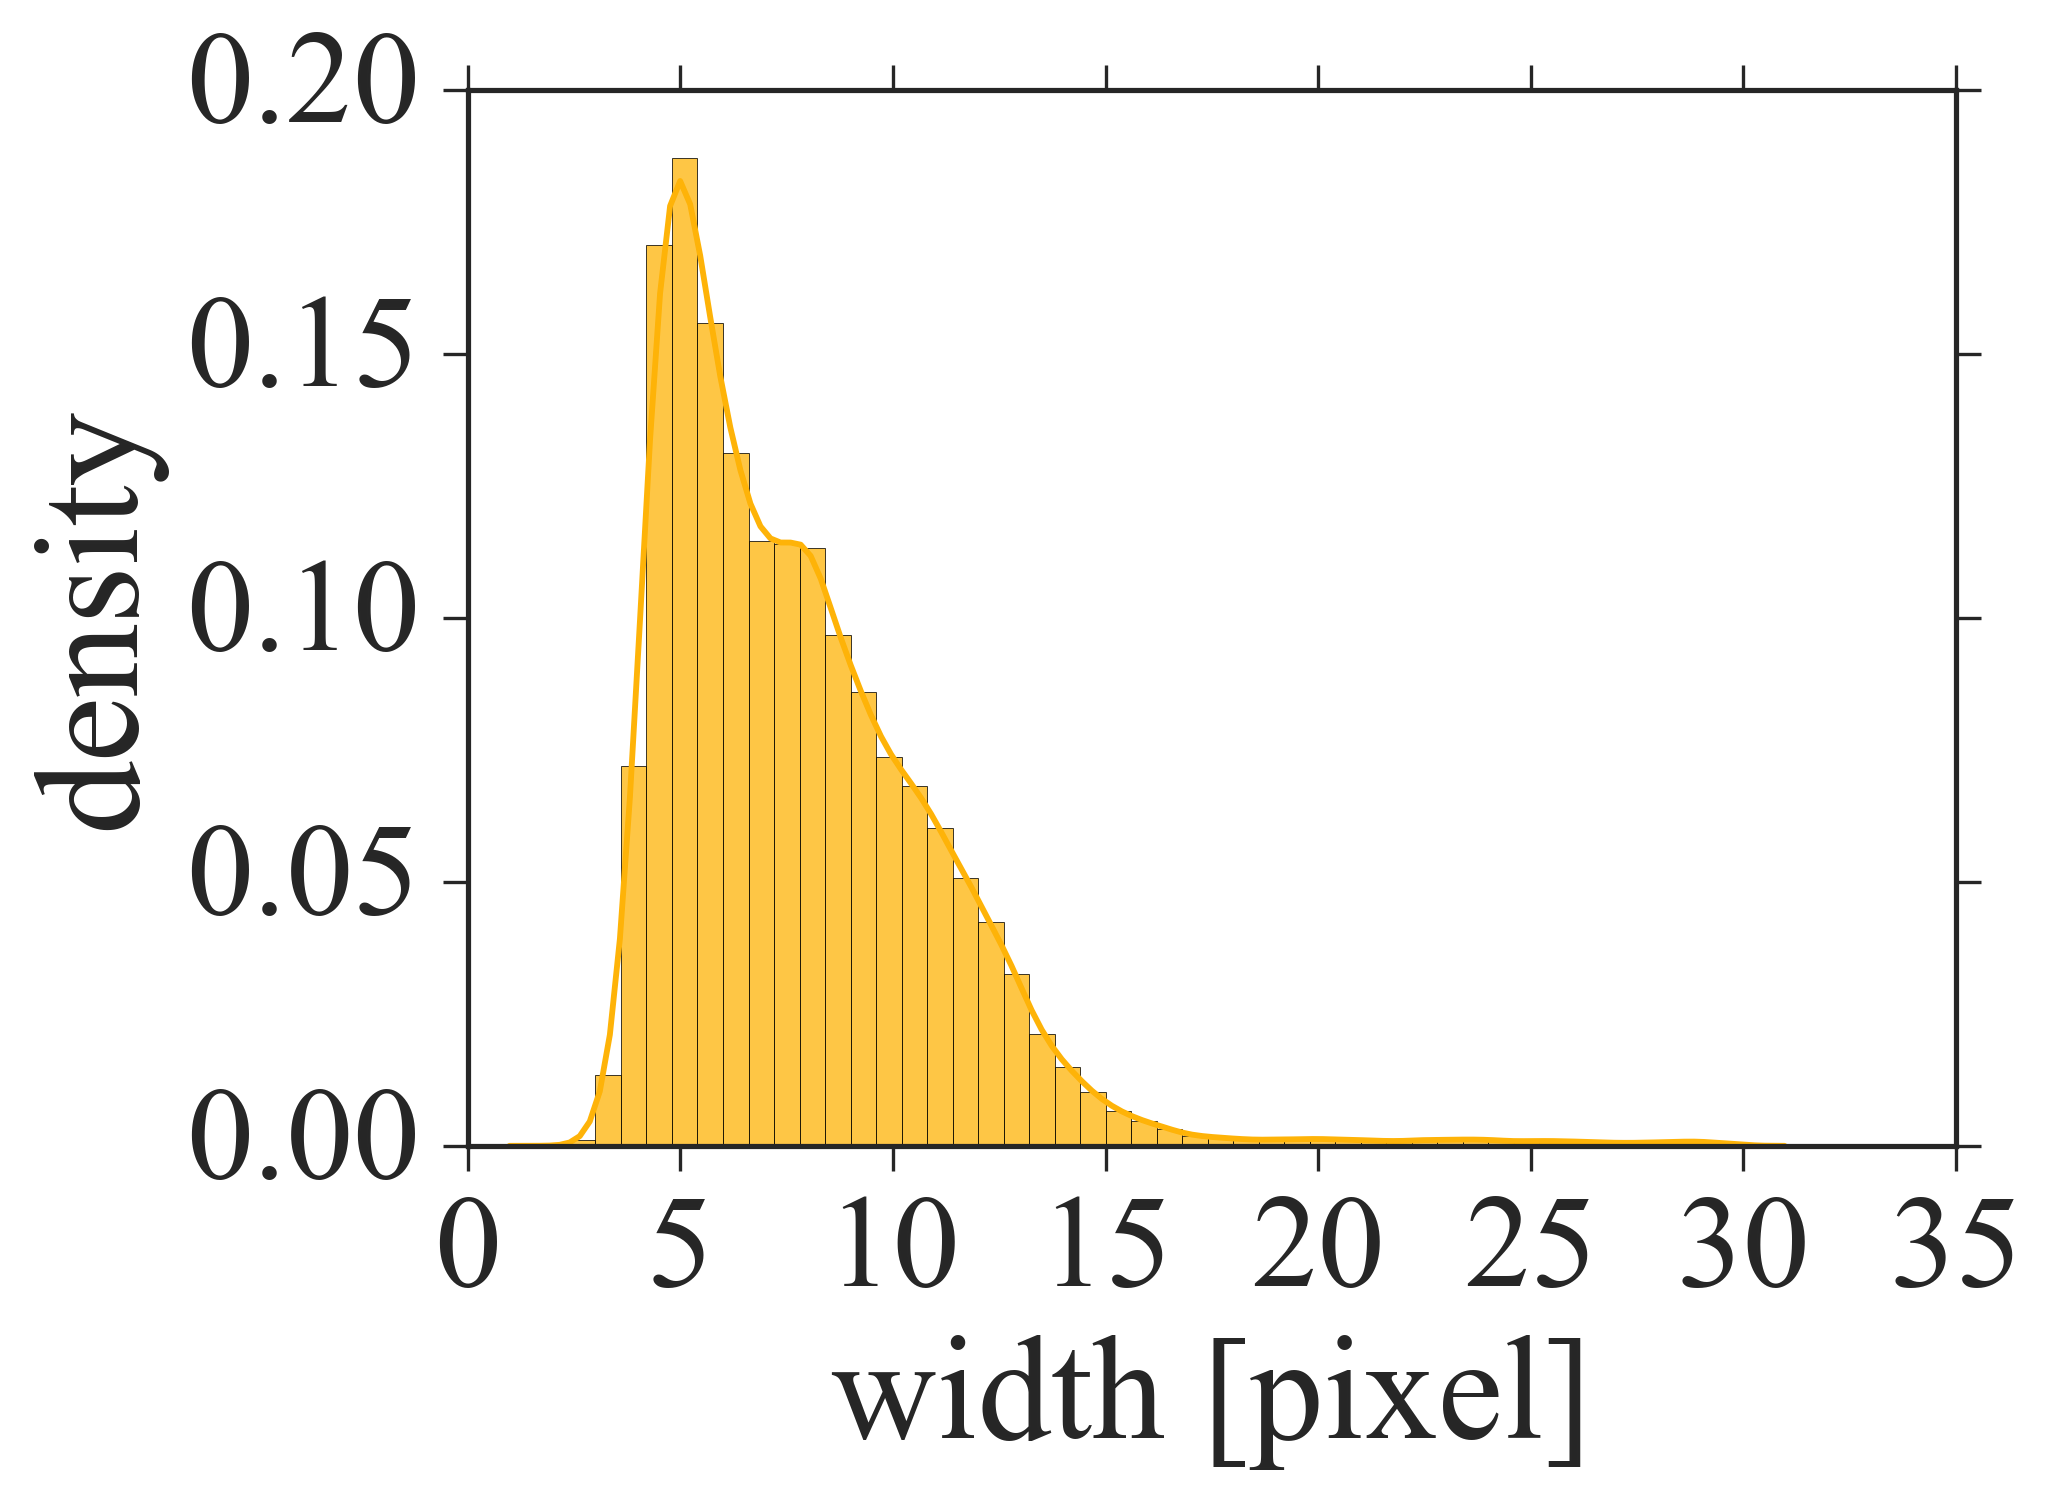
\includegraphics[width=0.45\textwidth]{demos/cummulative_edge_widths.png}}%
		\caption[Demo: How to compute an observable across an entire series of graphs.]{L.h.s.: A sample graph of \emph{P. polycephalum} from the \data. It is part of a series of $60$ graphs. R.h.s.: Cumulative edge width distribution computed over all $60$ graphs.}
    \end{figure}


	While computing such histograms is merely an exercise of using the information stored in the graphs, more interesting and insightful observables can be derived. In fact, in \Fref{chap:analysis} the results of a first systematic and in-depth study of the \data will be presented~\cite{dirnberger2016}.

	In the context of said study, additional questions that could be explored based on the \data naturally arose. In particular, one may determine whether there is a similarity between \emph{P.~polycephalum} networks and Voronoi graphs. The latter are well-studied and it is interesting to explore a possible connection between their properties and the features of \P. A different suggestion consists of answering the question whether \P graphs are geometric spanners. Spanners have properties that enable efficient communication between different parts of the graph, a feature clearly relevant and desirable for an organism such as \P.

	Yet another way to study the \data lies in the information provided by the tracking algorithm presented in this manuscript.	Since all the graphs in the data set already were tracked already, identifiers are available determining which nodes belong to which unique tracks. For simplicity, we refer to the track identifier as \emph{color}. As a proof-of-principle application, we shall demonstrate how to exploit this information to study the width of selected single edges in time. Since we aim to follow the time development of edges, we first need to establish the concept of tracks for edges. For any edge $e = (u,v)$, we define its color by combining the colors of $u$ and $v$ in a set:

	\begin{equation}
		\text{color}(e) = \{\text{color}(u), \text{color}(u)\}
	\end{equation}

	Looking at the tracking example given in \Fref{fig:tracking}, the edges $(b_1,e_1)$ and $(b_3,e_3)$ are assigned the color $\{blue, orange\}$ signaling that both edges belong to the same edge track and are merely different instances of one and the same edge at different points in time. Note that this edge is missing at $t=2$ and thus the length of the edge track is reduced by $1$.

	Given this edge color information it trivial to find all the edges that belong to an edge track. Once the tracks are known, it is easy to study how edge properties change within a track. \Fref{fig:unsplit} gives a detail of the graph shown in \Fref{fig:graph} and highlights two distinct edges which we want to investigate in this example. Edge $A$ was chosen such that the length of its track is equal to the length of the entire time series, \ie this thick edge is fully accounted for and does not disappear at any point in time. To illustrate the way the tracking algorithm resolves tracks where edges disappear at different points in time, we have selected an edge $B$ which is much thinner than $A$. There are two ways for an edge to disappear. Either its thickness falls below the detection threshold which means it is not present in the graph anymore, or it is split by the appearance of another edge. \Fref{fig:split} shows the latter situation where $B$ is split into two new edges by a newly detected third edge. The new edges have colors different from $B$.

	\begin{figure}
		\centering
        \subfloat[]{%
		\label{fig:unsplit}%
		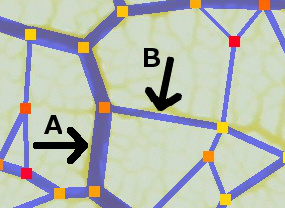
\includegraphics[width=0.45\textwidth]{demos/snipped_unsplit.JPG}}%
		\qquad
	    \subfloat[]{%
		\label{fig:split}%
		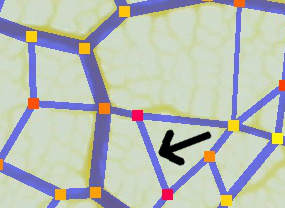
\includegraphics[width=0.45\textwidth]{demos/snipped_split.JPG}}%
		\caption[Demo: Setup for tracking of individual edges]{Details of a \emph{P. polycephalum} graph, see dashed rectangle in \Fref{fig:graph}. L.h.s.: Two edges $A$ and $B$ are selected for tracking. R.h.s.: A third edge appears, causing $B$ to split up and disappear from its track.}
    \end{figure}

    Finally, \Fref{fig:edge_tracking} shows the edge widths for edges $A$ and $B$ given their established tracks. Note that the track including the thicker edge $A$ runs across the entire $60$ graph in the series. The situation is different for edge $B$ where its track reflects that it is repeatedly split by a third edge which is sometimes present. Eventually, the splitting edge remains established for much of the latter half of the time series, thus superseding edge $B$ permanently. This simple example shows how the tracking information allows one to ``zoom in'' on what happens with selected edges and study them in detail.

    \begin{figure}
		\centering
		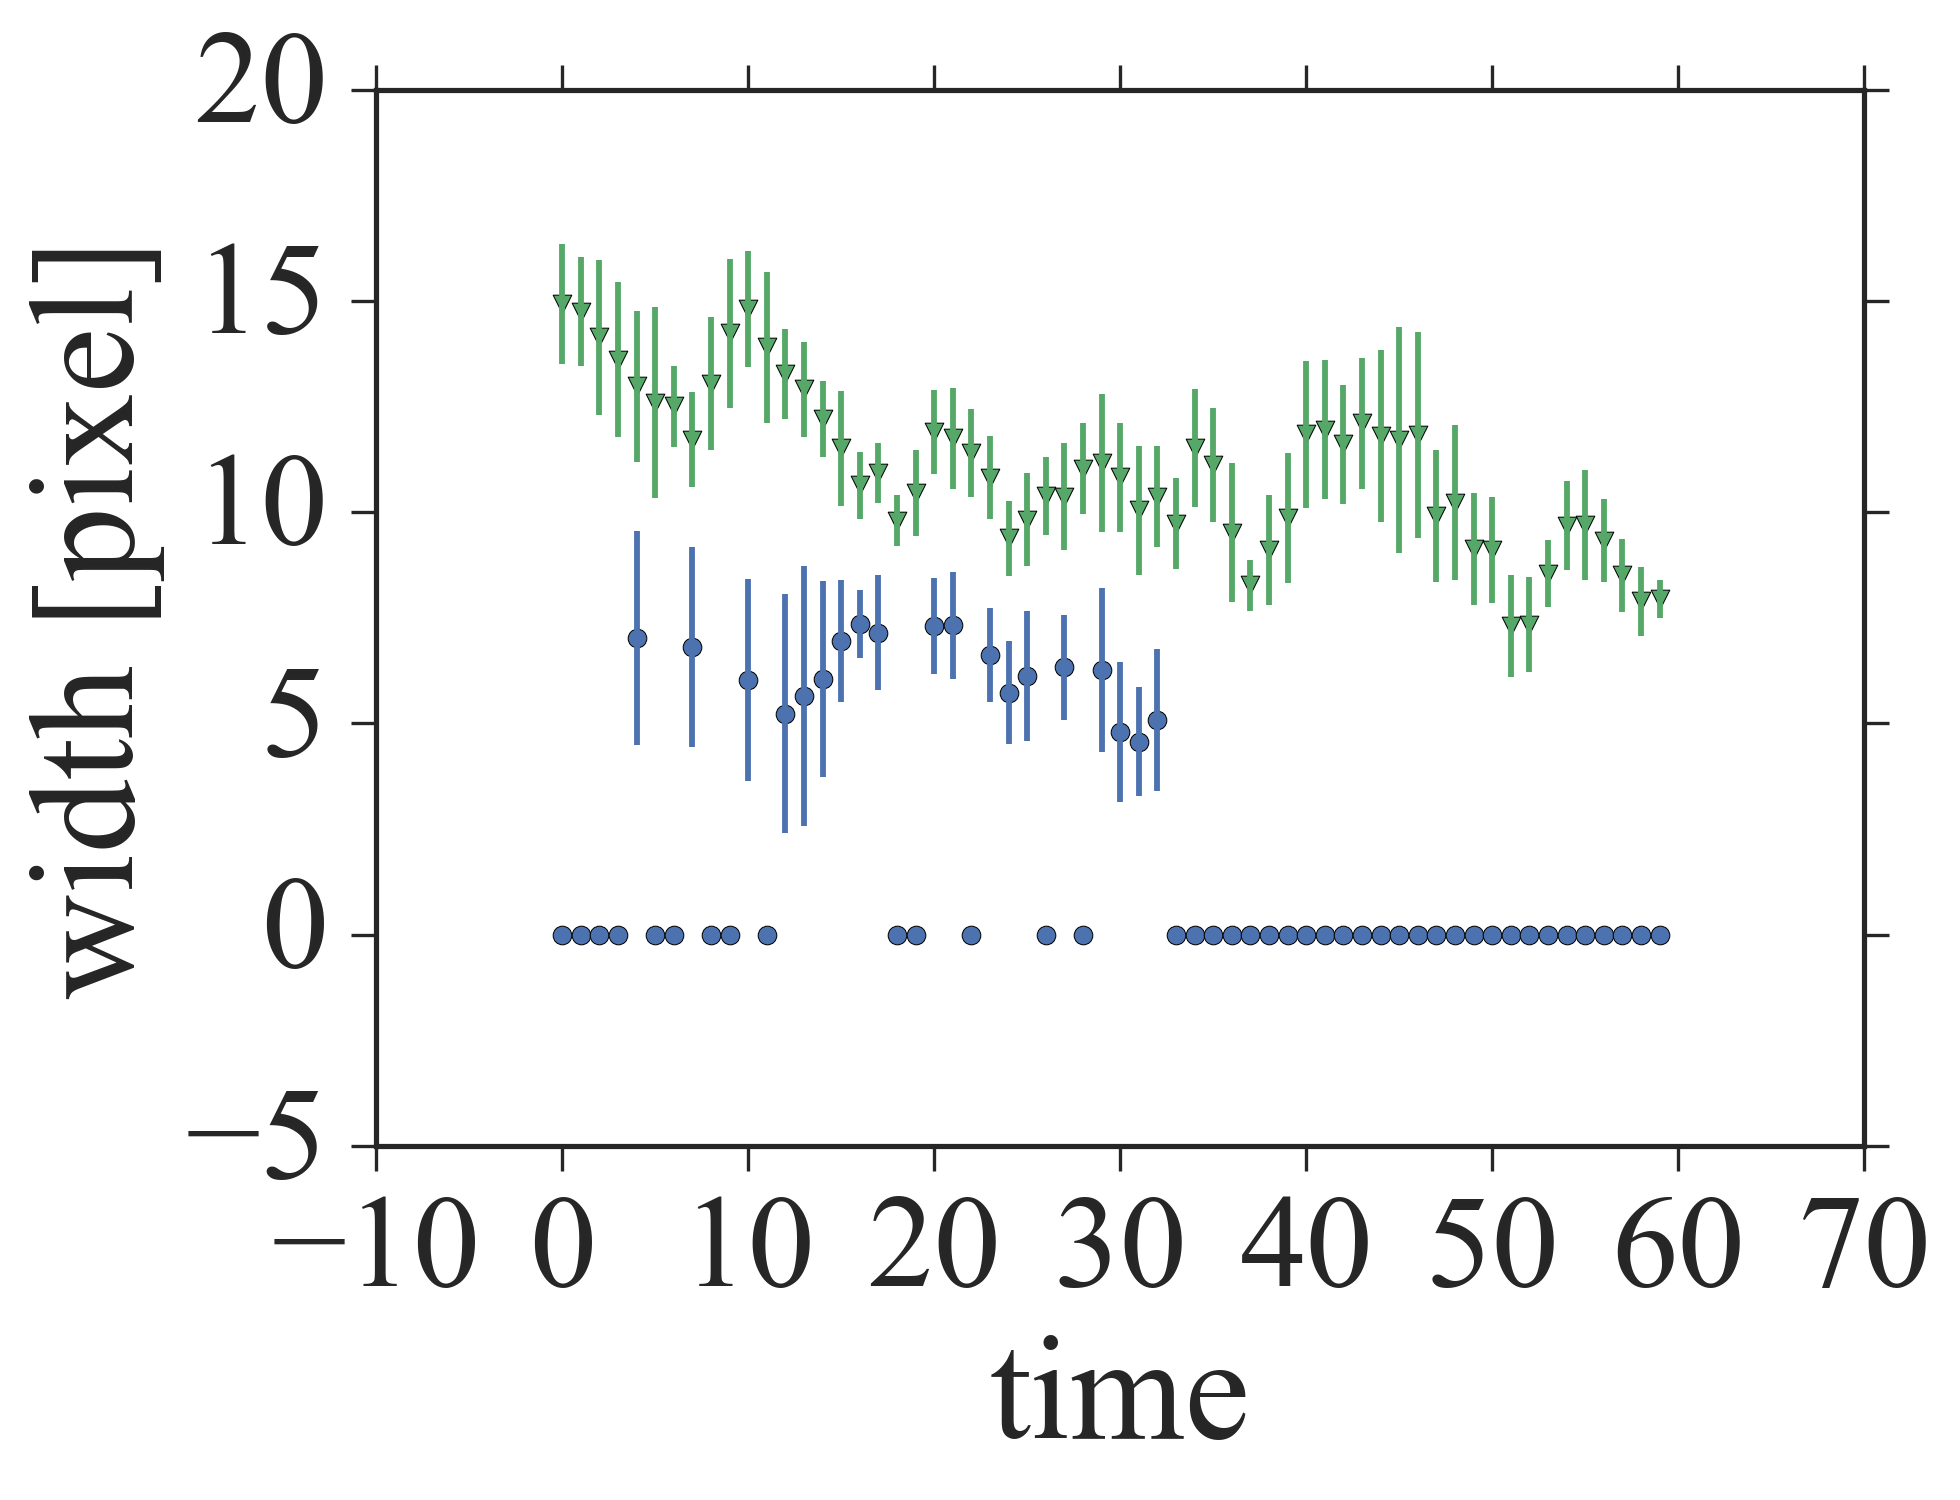
\includegraphics[width=0.60\textwidth]{demos/edge_tracking.png}%
		\caption[Demo: Results for tracking individual edges]{Development of edge widths for edges $A$ (green triangles) and $B$ (blue circles) as given by their established edge tracks. Note that for track $B$ we have set the value of the edge width to zero whenever the edge was missing. This serves to illustrate the fragmentation of rack $B$ compared to track $A$. The widths are given in units of pixel and time is measured in units of \SI{120}{\second}.}
		\label{fig:edge_tracking}%
    \end{figure}


	At the time of writing this manuscript the novel information provided by the computed tracking is yet to be explored in a large and systematic study. What can be inferred from the topological changes recorded? Can one identify patterns with certain structural properties? Can topological properties be related to questions of biological relevance? Given the large number of graphs in the \SMGR, an investigation of such questions becomes viable as future research.

	The \data is not limited to the use cases and suggestions provided below. Rather, they constitute a flexible basis to work with as it contains a host of useful data, code and instructions. In particular, potential users are not restricted to working with the graphs that are presently provided. They are encouraged to start from the raw images and determine their own specific data selection, graph extraction and tracking procedures tailored to their particular research agenda. They may use the tools provided by us or deploy entirely different strategies to better suit their needs.

\section{Discussion}

	The first and most important step in sharing your data is to share your data~\cite{white2013nine}. To this end, we introduce the Slime Mold Graph Repository, a novel platform that facilitates the exchange of experimental data revolving around networks formed by slime molds. We believe that by encouraging the reuse of data, the value and visibility of experimental ground work is significantly increased. Not only does the reproduction of results based on publicly available data become much easier, shared data may be put to unforeseen use by researchers from different fields willing to examine it from a new point of view.

	To enable this, we initiate the \SMGR with an extensive set of raw data, ready-to-use graphs and dedicated methods such as the introduced tracking algorithm. We show the usefulness of time-series of graphs by discussing two out of many possible different approaches to investigate them. First, we discuss how to obtain simple statistical observables for all edges in the graph. In particular, we compute the cumulative distribution of edge widths. Second, we illustrate how the information obtained by the tracking algorithm allows us to explore the time-development of single edges.

	Clearly, future investigations are hardly limited to the examples and suggestion given in this manuscript. It is fair to say that any observable defined on a weighted graph, relevant to \P, can be studied using the \data. In particular, we'd like to stress the implications for evaluating and guiding all sorts of theoretical modeling approaches based on graphs. Any model that produces a prediction which can be formulated as an observable defined on a graph can immediately be tested on the \data. This includes time dependent observables. Predictions that agree with \SMGR data may increase the trust in a given model, while discrepancies between predictions and data hopefully suggest improvements. Thus, data contained in the \data may be used to drive modeling efforts and help bridge the gap between theory and experiment.

	We would like the research community to interpret the \SMGR as a twofold challenge. First, we challenge people working on slime molds to contribute their data, enable others and to increase the visibility and impact of their experimental work at the same time. Second, we challenge everyone to use the current contents of the \SMGR and to come up with new ways to enrich our understanding of the interesting organisms that are slime molds.
	   
\section{Acknowledgments}

	We are grateful to Prof.~T.~Ueda for providing us with sclerotia and for teaching us to the art of culturing \Pp with infinite patience. We thank Prof.~M.~Grube and Dr.~C.~Westendorf for hospitality, support and expert advice on slime molds. We acknowledge Prof.~A.~Manz and Prof.~L.~Abelmann and their group at \href{www.kist-europe.de}{\textsc{Kist} Europe} for stimulating discussions. Lastly, we are grateful towards Dr.~M.~F\"ugger for his encouraging comments and proof-reading.
